\documentclass[pdftex]{beamer}
\usepackage{amssymb,amsmath,mathrsfs}
\usecolortheme{default}

% this one is debatable
\renewcommand{\emph}[1]{\textbf{#1}}

%%% color commands
\newcommand{\whiteonblack}{%
  \colorlet{fg}{white}
  \colorlet{bg}{black}
  \setbeamercolor{normal_text}{fg=white,bg=black}
  \setbeamercolor{background canvas}{fg=white,bg=black}
  \setbeamercolor{alerted_text}{fg=yellow}
  \setbeamercolor{example_text}{fg=white}
  \setbeamercolor{structure}{fg=white}
  \setbeamercolor{palette_quaternary}{fg=white}
}
\newcommand{\blackonwhite}{%
  \colorlet{fg}{black}
  \colorlet{bg}{white}
  \setbeamercolor{normal_text}{fg=black,bg=white}
  \setbeamercolor{background canvas}{fg=black,bg=white}
  \setbeamercolor{alerted_text}{fg=blue}
  \setbeamercolor{example_text}{fg=black}
  \setbeamercolor{structure}{fg=black}
  \setbeamercolor{palette_quaternary}{fg=black}
}
\xdefinecolor{pink}{rgb}{1.0,0.9,0.9}

%%% size and shape commands
\newlength{\figurewidth}
\setlength{\figurewidth}{0.9\textwidth}
\newlength{\figureheight}
\setlength{\figureheight}{0.9\textheight}

%%% text commands
\newcommand{\project}[1]{\textsl{#1}}
  \newcommand{\an}{\project{Astrometry.net}}
  \newcommand{\euclid}{\project{Euclid}}
  \newcommand{\flickr}{\project{flickr}}
  \newcommand{\gaia}{\project{Gaia}}
  \newcommand{\galex}{\project{GALEX}}
  \newcommand{\kepler}{\project{Kepler}}
  \newcommand{\GALEX}{\galex}
  \newcommand{\hst}{\project{HST}}
  \newcommand{\hipparcos}{\project{Hipparcos}}
  \newcommand{\lsst}{\project{LSST}}
  \newcommand{\sdss}{\project{SDSS}}
  \newcommand{\sdssiii}{\project{SDSS-III}}
  \newcommand{\sdssiv}{\project{SDSS-IV}}
  \newcommand{\boss}{\project{BOSS}}
  \newcommand{\apogee}{\project{APOGEE}}
  \newcommand{\osss}{\project{OSSS}}
  \newcommand{\ska}{\project{SKA}}
  \newcommand{\vo}{\project{VO}}
  \newcommand{\rttd}{\project{Right Thing To Do}$^{\mbox{\scriptsize\sffamily{TM}}}$}
\newcommand{\foreign}[1]{\textit{#1}}
\newcommand{\latin}[1]{\foreign{#1}}
  \newcommand{\cf}{\latin{cf.}}
  \newcommand{\eg}{\latin{e.g.}}
  \newcommand{\etal}{\latin{et~al.}}
  \newcommand{\etc}{\latin{etc.}}
  \newcommand{\ie}{\latin{i.e.}}
  \newcommand{\vs}{\latin{vs.}}

%%% math-mode commands
\newcommand{\unit}[1]{\mathrm{#1}}
  \newcommand{\rad}{\unit{rad}}
  \newcommand{\s}{\unit{s}}
  \newcommand{\yr}{\unit{yr}}
  \newcommand{\km}{\unit{km}}
  \newcommand{\kmps}{\km\,\s^{-1}}
\newcommand{\mmatrix}[1]{\boldsymbol{#1}}
\newcommand{\tv}[1]{\boldsymbol{#1}}
\newcommand{\dd}{\mathrm{d}}
\newcommand{\given}{\,|\,}
 % hogg standard colors
\input{vc}
\setlength{\paperheight}{3.5in}
% 1.77778 is the ratio of 16 to 9
\setlength{\paperwidth}{1.77778\paperheight}
% 1.33333 is the ratio of 4 to 3
% \setlength{\paperwidth}{1.33333\paperheight}
\setlength{\textwidth}{0.85\paperwidth}
\usepackage{amssymb,amsmath,mathrsfs}

\title{Data-driven models of stars}
\author[David W. Hogg (NYU)]{David W. Hogg \\
  \textsl{\small Center for Cosmology and Particle Physics,
                 New York University}}
\date{2015 January 20}

\begin{document}

\begin{frame}
  \titlepage
  \texttt{\giturl~\githash~(\gitdate)} \\
  in collaboration with \emph{Melissa Ness} (MPIA) and Hans-Walter Rix
\end{frame}

\begin{frame}
  \frametitle{The paradox of precision astrophysics}
  \begin{itemize}
  \item models are incredibly explanatory
  \item models are wrong (ruled out) in detail
    \begin{itemize}
    \item $\Lambda$CDM
    \item stellar spectroscopy
    \item helioseismology
    \end{itemize}
  \item approximations, computation, gastrophysics
  \end{itemize}
\end{frame}

\begin{frame}
  \frametitle{physics-driven models}
  \begin{itemize}
  \item put in everything you know
  \item make approximations to make things computable
  \end{itemize}
\end{frame}

\begin{frame}
  \frametitle{machine learning}
  \begin{itemize}
  \item the most extreme of data-driven models
  \item ``the data \emph{is} the model''
    \begin{itemize}
    \item none of your knowledge is relevant
    \end{itemize}
  \item learn (fit) an exceedingly flexible model
    \begin{itemize}
    \item explain or cluster the data
    \item transformation from data to ``labels''
    \end{itemize}
  \item concept of non-parametrics
  \item concept of train, validate, and test
  \item many packages and implementations to choose from
    \begin{itemize}
    \item (and outrageous successes)
    \end{itemize}
  \end{itemize}
\end{frame}

\begin{frame}
  \frametitle{data-driven models}
  \begin{itemize}
  \item \textit{(my personal usage)}
  \item make use of things you \emph{strongly believe}
    \begin{itemize}
    \item noise model \& instrument resolution
    \item causal structure (shared parameters)
    \end{itemize}
  \item capitalize on huge amounts of data
  \item exceedingly flexible model
  \item concept of train, validate, and test
  \item every situation will be \emph{bespoke}
  \end{itemize}
\end{frame}

\begin{frame}
  \frametitle{when does machine learning help you?}
  \begin{itemize}
  \item train \& test situation
  \item training data are statistically identical to the test data
    \begin{itemize}
    \item same noise amplitude
    \item same distance or redshift distribution
    \item same luminosity distributionn
    \item \emph{never true!}
    \end{itemize}
  \item (training data have accurate and precise labels)
  \item we \emph{can't use vanilla machine learning!}
  \end{itemize}
\end{frame}

\begin{frame}
  \frametitle{Why stellar parameters and chemical abundances?}
  \begin{itemize}
  \item top priority for many new projects
    \begin{itemize}
    \item \gaia
    \item \project{HERMES} \& \project{GALAH}
    \item \sdssiii\ \apogee
    \end{itemize}
  \item extended distribution functions
  \item chemical tagging
    \begin{itemize}
    \item the dynamics and formation of the Milky Way
    \end{itemize}
  \end{itemize}
\end{frame}

\begin{frame}
  \frametitle{\sdssiii\ \apogee}
  \begin{itemize}
  \item foo
  \item foo
    \begin{itemize}
    \item bar
    \item bar
    \end{itemize}
  \item foo
  \end{itemize}
\end{frame}

\newcommand{\credits}{{\footnotesize (Ness, Hogg, Rix, \etal)}}
\newcommand{\teff}{T_{\mathrm{eff}}}
\newcommand{\logg}{\log g}
\newcommand{\feh}{[\mathrm{Fe / H}]}

\begin{frame}
  \frametitle{\tc\ \credits: training set}
  \begin{itemize}
  \item 543 stars (too few) from 19 clusters (too few)
  \item $\teff, \logg, \feh$ labels from \apogee
    \begin{itemize}
    \item calling parameters and abundances ``labels''
    \item slight adjustments to labels to get them onto possible isochrones
    \end{itemize}
  \item \emph{terrible} coverage of the main sequence
    \begin{itemize}
    \item only the Pleiades
    \item home-made Pleiades labels (by Ness)
    \end{itemize}
  \end{itemize}
\end{frame}

\begin{frame}
  \frametitle{\tc\ \credits: training set}
  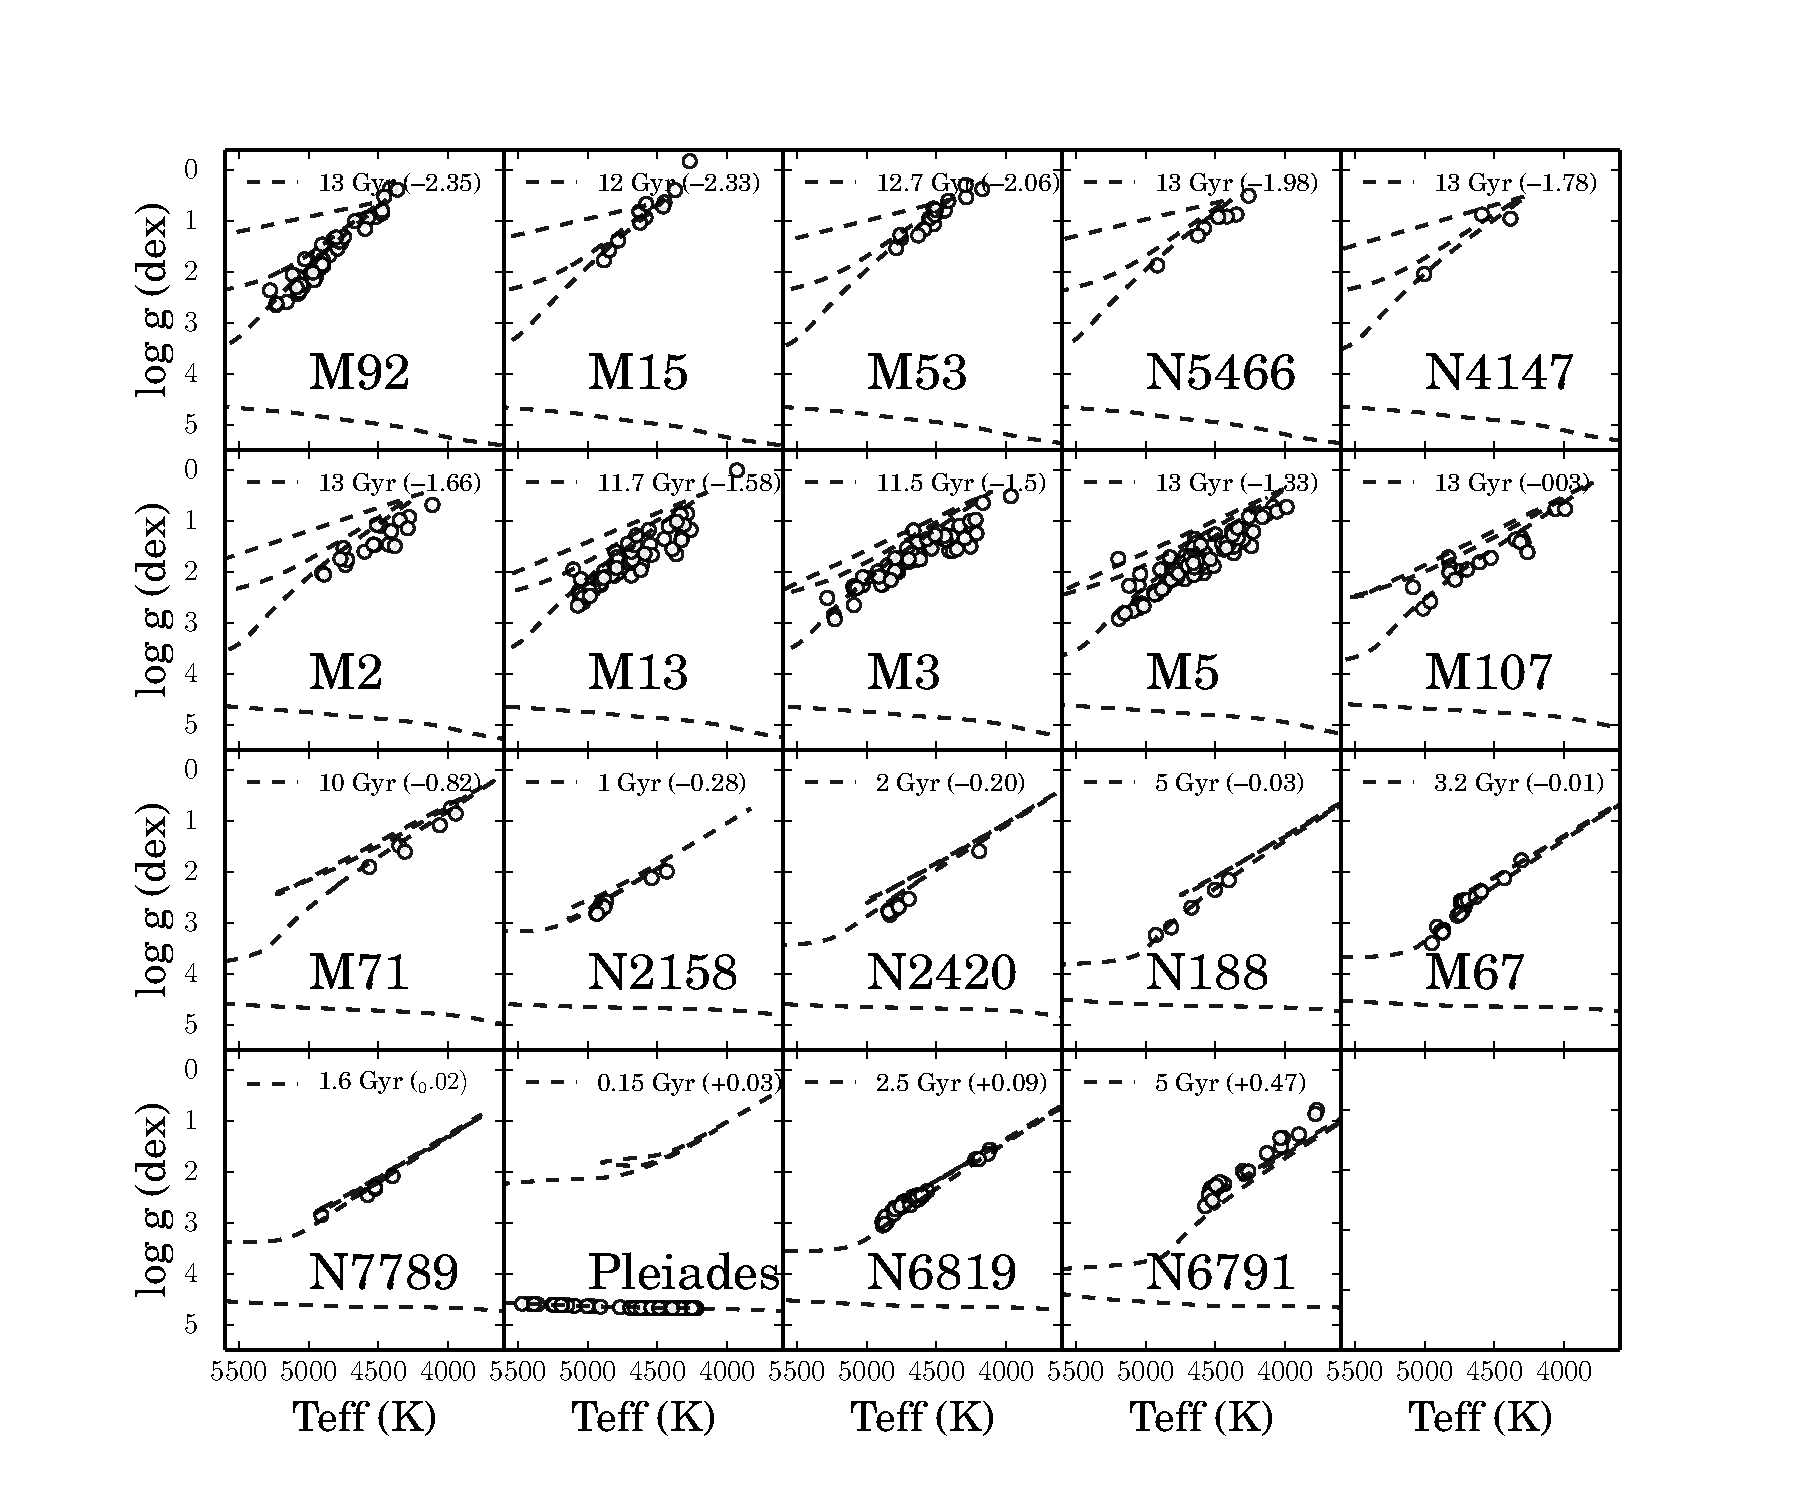
\includegraphics[height=0.9\textheight]{../documents/plots/training_aspcap2.pdf}
\end{frame}

\newcommand{\flux}{f}
\newcommand{\fluxes}{\boldsymbol{\flux}}
\newcommand{\labels}{\boldsymbol{\ell}}
\newcommand{\pars}{\boldsymbol{\theta}}

\begin{frame}
  \frametitle{\tc\ \credits: model}
  \begin{itemize}
  \item a \emph{generative model} of the \apogee\ spectra
    \begin{itemize}
    \item given label vector $\labels$, predict flux vector $\fluxes$
    \item probabilistic prediction $p(\fluxes\given\labels,\pars)$
    \end{itemize}
  \item use every spectral pixel's uncertainty variance $\sigma^2_{\lambda n}$ responsibly
  \item details:
    \begin{itemize}
    \item spectral expectation is quadratic in the labels
    \item every wavelength $\lambda$ treated independently
    \item an intrinsic Gaussian scatter $s^2_\lambda$ at every wavelength $\lambda$
    \end{itemize}
  \end{itemize}
\end{frame}

\begin{frame}
  \frametitle{\tc\ \credits: model}
  \begin{eqnarray}
    \ln p(\fluxes_n\given\labels_n,\pars) &=& \sum_\lambda \ln p(\flux_{\lambda n}\given\labels_n,\pars_\lambda) \\
    \ln p(\flux_{\lambda n}\given\labels_n,\pars_\lambda) &=& -\frac{1}{2}\,\frac{[\transpose{\pars_\lambda}\cdot\labels_n]^2}{\sigma^2_{\lambda n} + s^2_\lambda} \\
    \labels_n &\equiv& \left[1, \teff, \logg, \feh, \teff^2, \teff\,\logg, \cdots, \feh^2\right] \\
  \end{eqnarray}
  \begin{itemize}
  \item \emph{training step}: optimize parameters $\pars$ at fixed labels
    $\labels$ using training-set data
  \item \emph{test step}: optimize labels $\labels$ at fixed
    parameters $\pars$ using test-set (survey) data
  \end{itemize}
\end{frame}

\begin{frame}
  \frametitle{\tc\ \credits: results}
  \begin{itemize}
  \item foo
  \item foo
    \begin{itemize}
    \item bar
    \item bar
    \end{itemize}
  \item foo
  \end{itemize}
\end{frame}

\begin{frame}
  \frametitle{\tc\ \credits: shortcuts and choices}
  \begin{itemize}
  \item foo
  \item foo
    \begin{itemize}
    \item bar
    \item bar
    \end{itemize}
  \item foo
  \end{itemize}
\end{frame}

\begin{frame}
  \frametitle{other applications for data-driven models}
  \begin{itemize}
  \item foo
  \item foo
    \begin{itemize}
    \item bar
    \item bar
    \end{itemize}
  \item foo
  \end{itemize}
\end{frame}

\begin{frame}
  \frametitle{conservatism requires huge numbers of parameters}
  \begin{itemize}
  \item foo
  \item foo
    \begin{itemize}
    \item bar
    \item bar
    \end{itemize}
  \item foo
  \end{itemize}
\end{frame}

\end{document}
